\documentclass{ctexart}
\usepackage[hmargin=1.1in,vmargin=1in]{geometry}
\usepackage{amsmath}
\usepackage{graphicx}
\usepackage[defaultmono]{droidsansmono}

\title{《信号处理导论》课程报告二}
\input{personal_info/info.tex}

\begin{document}
    \maketitle

    \section{我学到了哪个知识点?}

    广义函数。尽管形式上,广义函数与普通一元函数一样,都使用 \verb|<函数名>(<自变量名>)| 的记号,都接受一个数字
    自变量。但实际上,广义函数的操作对象是一类普通函数。与一般函数将一个数映射到另一个数上相不同,广义函数将一个函数
    映射到一个数上。

    更确切地说,广义函数 $g(t)$ 指的是这样的函数:取一合适的\textbf{普通函数}集 $S$,对任意函数 $f(t) \in S$,有

    \[
        -\infty < \int_{-\infty}^{+\infty} g(t) \cdot f(t) \mathrm{d}t = N[g(t), f(t)] < +\infty
    \]

    其中普通函数 $f(t)$ 称为检验函数,集合 $S$ 称为检验函数空间,$N = N[g(t), f(t)]$ 就是广义函数 $g(t)$ 将
    普通函数 $f(t)$ 映射到数域上的像。特别地,检验函数可以是常函数(即 $f(x) = C$,$C$ 为一常数)。

    来源:《信号与线性系统分析》第四版——吴大正 1.4 节 阶跃函数与冲激函数。

    \section{我之前是怎么想的?}

    函数就是函数,将一个“数”映射成另一个“数”,因此被称为函“数”。高等数学中倒是引入了一些诸如“二元函数”等的概念,但是
    在定义域内,一个函数仍然是将一个(或者几个)数映射到一个有限大小的数上。因此对于一个给定的自变量取值 $x = x_0$,
    函数的值 $f(x)$ 必是确定且有穷的(虽然不一定可精确求出解析解)。高数中也有定义过一些其它的操作,比如导数等,能够
    将某一个函数“映射”成另一个函数,但这些本质上只是一些针对函数的“变形操作”,不属于“函数”。

    \section{我之前的想法怎么样?}

    一种“传统”的认知。在中学阶段,这种认知是正确的,但是在进入更高等级的学习之后,这种认知就显得``不够用''了。

    \section{我应该怎样想才对?}

    类似于虚数/复数是对数(实数)的扩充一样,广义函数是对函数的扩充(广义函数仍然属于映射:它将检验函数空间内的每一个
    函数都映射到一个数上)。大多数时候,初等函数或者分段、不连续的初等函数已经足够用来描述很多的事物,但是有些时候,
    比如说``处处连续,但是在某一个或几个时间点附近以几乎为 0 的时间从一个值变化到另一个值''就无法再用``传统的函数''
    来表达。此时,我们就可以引入``广义函数''来方便地描述这些函数,比如单位冲激函数 $\delta(x) $可以定义为
    $\int \limits_{-\infty}^{+\infty} \delta(x) \cdot \varphi(x) = \varphi(0)$。

    \section{我应该怎样用上它?}

    ``广义函数''的概念让我想到之前学程序设计时听说的,一个叫做``高阶函数''的概念。高阶函数是一类函数(程序设计意义上),
    它们接受至少一个,或者返回一个函数。最有名的高阶函数是 \verb|map| 函数与 \verb|reduce| 函数,它们都接收一个函数
    $f$ 和一个序列 $S$ 作为参数,并将 $f$ 作用于 $S$ 的各个元素上,具体来说:

    \begin{itemize}
        \item \verb|map| 返回一个序列 $S' = \{f(S_1), f(S_2), \ldots, f(S_n)\}$;
        \item \verb|reduce| 返回一个元素 $v = f(f(f(f(S_1, S_2), S_3), \ldots), S_n)$。
    \end{itemize}

    另一方面,广义函数又和概率论中的概率密度函数很像(式中 $f(x)$ 是随机变量 $X$ 的概率密度函数,$g(X)$ 是随机变量
    $X$ 的函数):

    \[
        \mathrm{E} g(X) = \int\limits_{-\infty}^{+\infty} g(x)\cdot f(x) \mathrm{d}x
    \]

    由此,我们也可以认为概率密度函数 $f(X)$ 实质上也是一个高阶函数 $f(g) = \mathrm{E} g(X)$。

    \section*{字数统计}

    \begin{center}
        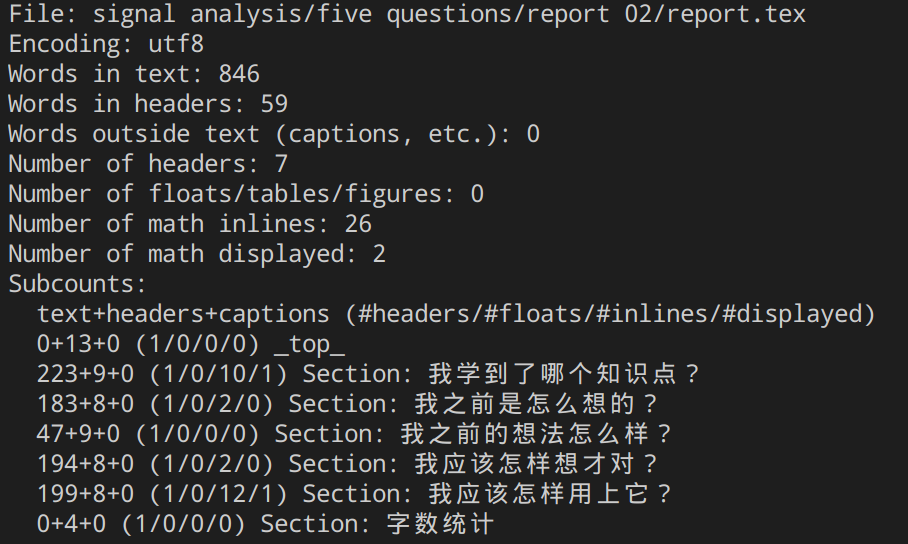
\includegraphics[width=0.7\textwidth]{pics/texcount.png}
    \end{center}

\end{document}